%!TEX root =  ../main.tex

\mychapters{Probabilities}{probability}{\chapdir/pics/1280px-13-02-27-spielbank-wiesbaden-by-RalfR-093} 
What are the chances?

\newpage
\chapterminitoc

%									14 - 1
\newpage
\section{Chances}
\subsection{Two Dice}
\noindent\makebox[\textwidth]{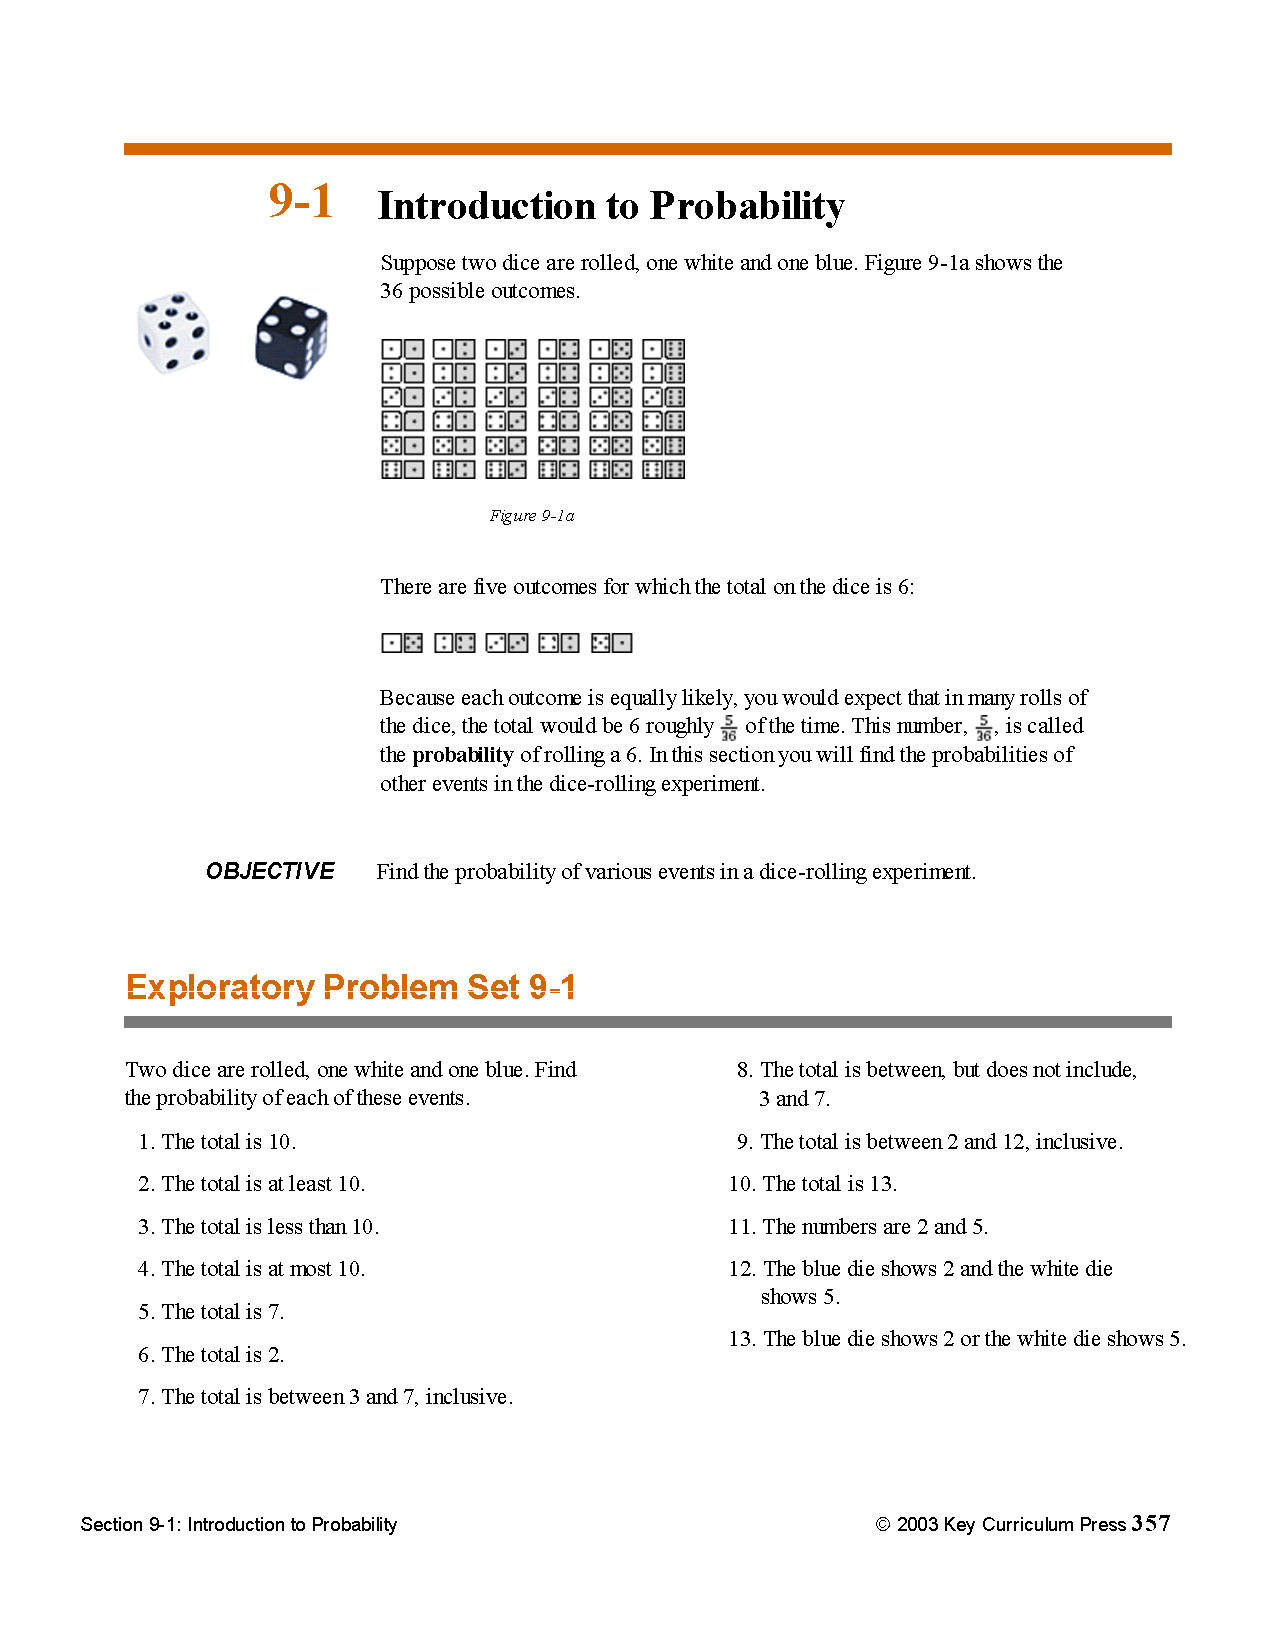
\includegraphics[width=\paperwidth]{ch14/1401p.pdf}}
\subsection{Rule of Product}
\personfeature{\chapdir/pics/Pierre_de_Fermat.jpg}{Pierre de Fermat}{1607-1665}{was a French mathematician who is given credit for early developments that led to infinitesimal calculus,  analytic geometry, probability, and optics. \href{https://en.wikipedia.org/wiki/Pierre_de_Fermat}{Wikipedia}}
\subsection{Combinatorics}
\subsection{Exercises}

%									14 - 2
\newpage
\section{Counting Principle}
\subsection{Clusivity}
\noindent\makebox[\textwidth]{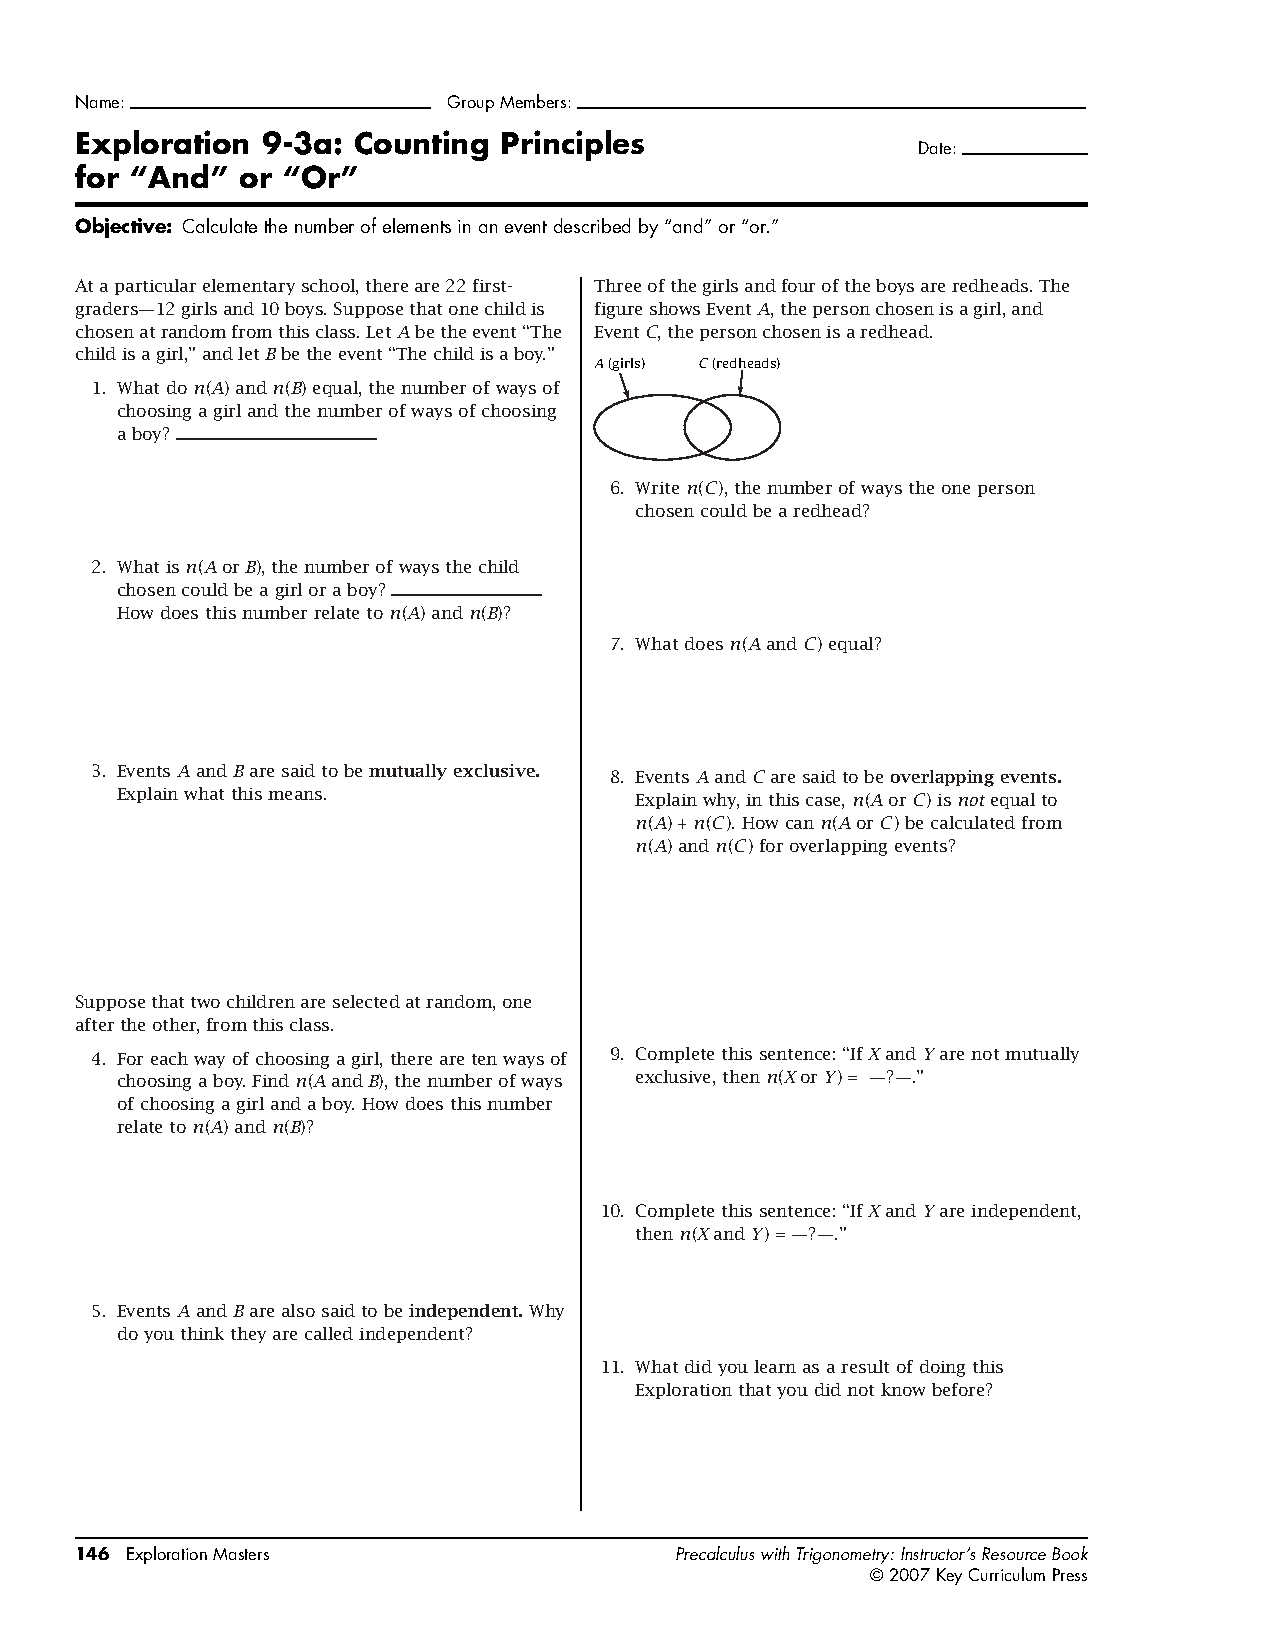
\includegraphics[width=\paperwidth]{ch14/1402p.pdf}}
\subsection{Logical AND and OR}
\subsection{Factorial}
\subsection{Exercises}

%									14 - 3
\newpage
\section{Permutation}
\noindent\makebox[\textwidth]{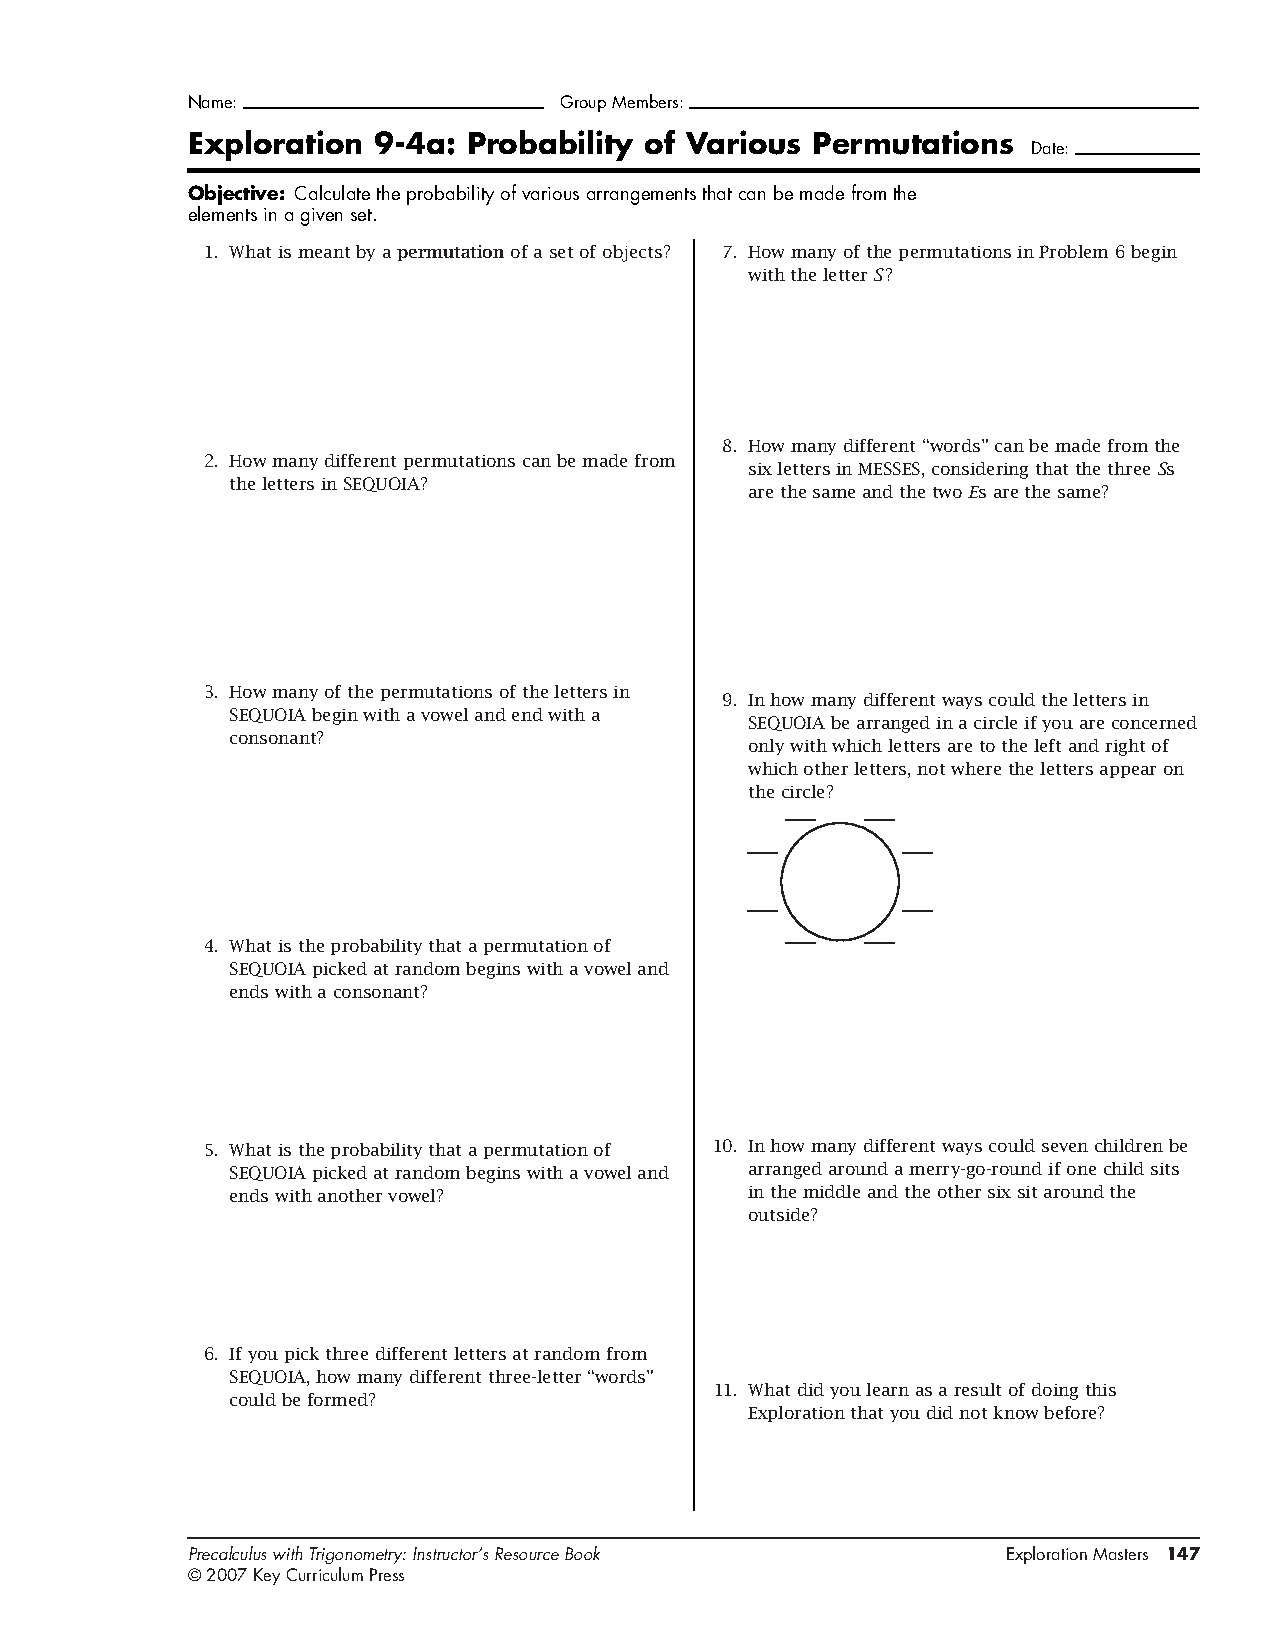
\includegraphics[width=\paperwidth]{ch14/1403p.pdf}}
\subsection{$_nP_r$}
\subsection{Circular Arrangements}
\subsection{Exercises}

%									14 - 4
\newpage
\section{Combination}
\noindent\makebox[\textwidth]{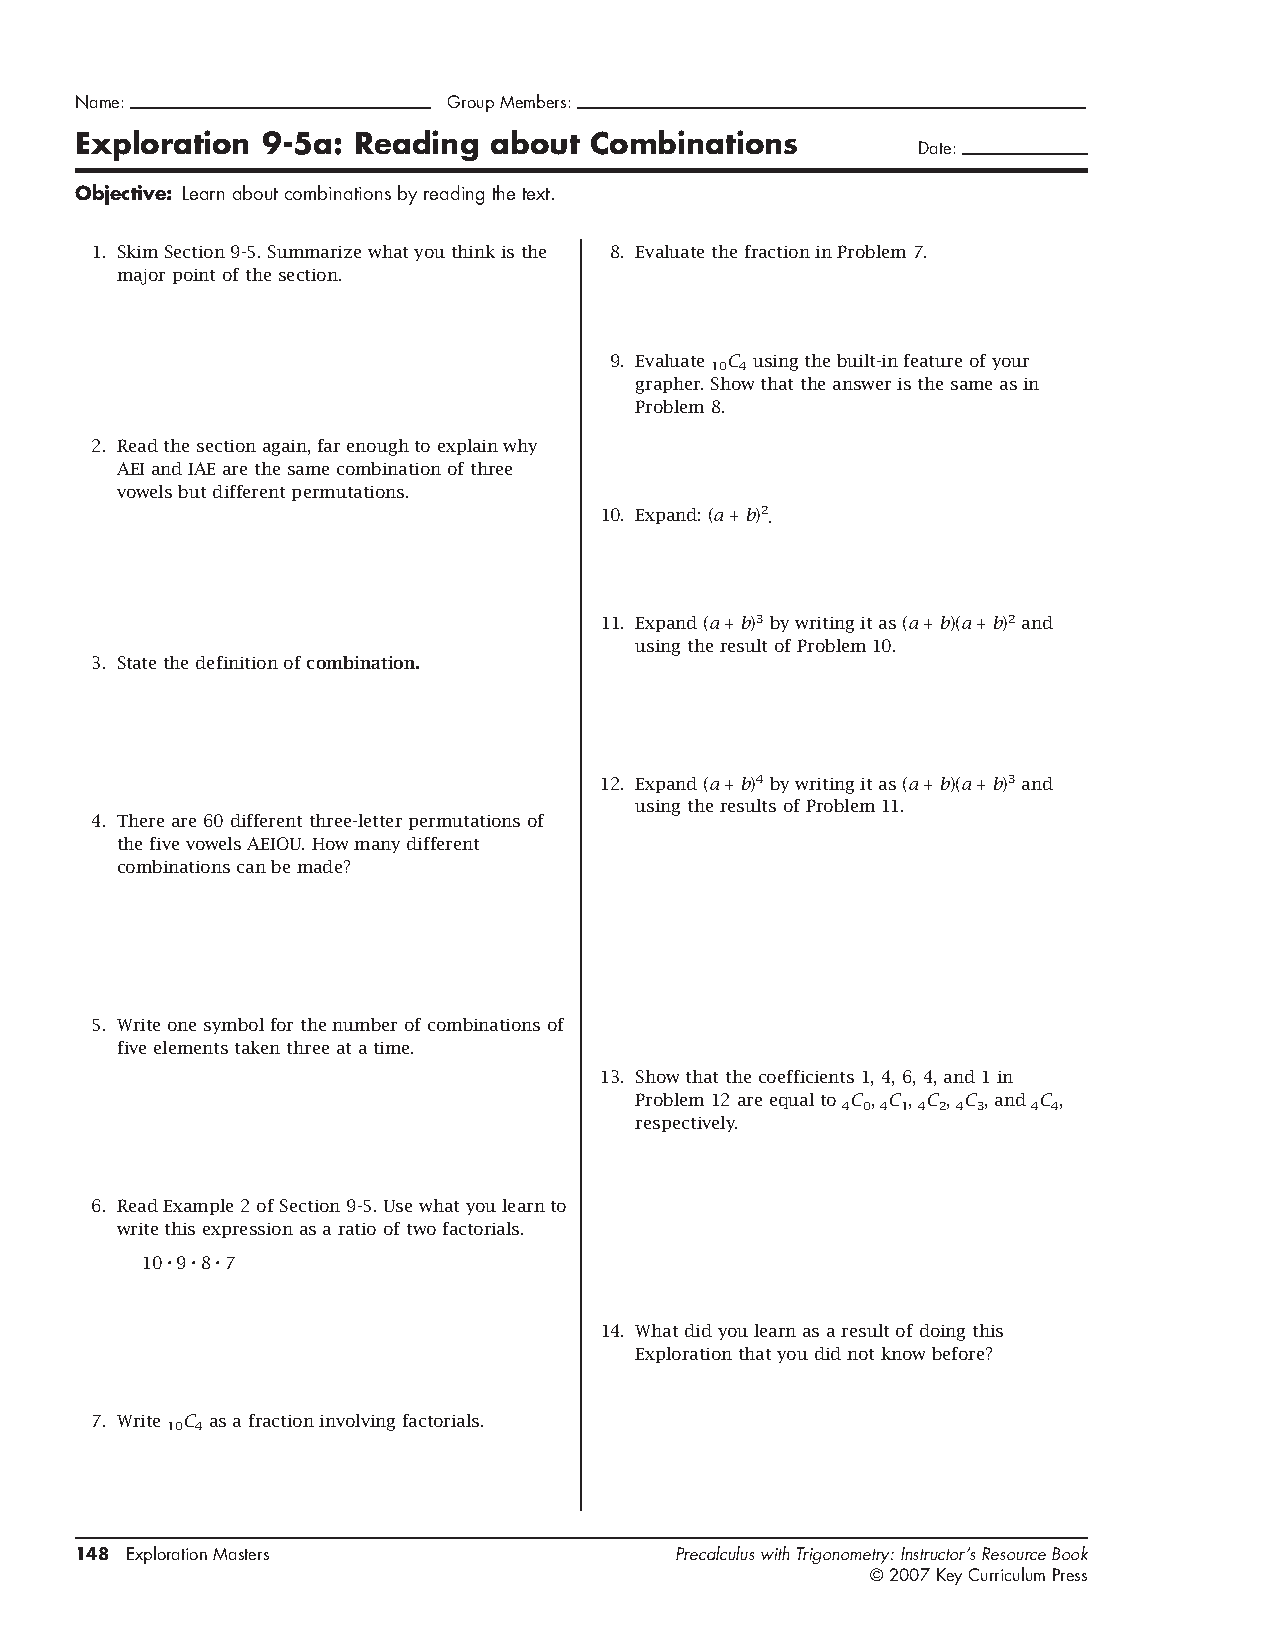
\includegraphics[width=\paperwidth]{ch14/1404p.pdf}}
\subsection{$_nC_r$}
\subsection{n Choose r}
\subsection{Pascal's Triangle}
\subsection{Exercises}

%									14 - 5
\newpage
\section{Binomial Series}
\noindent\makebox[\textwidth]{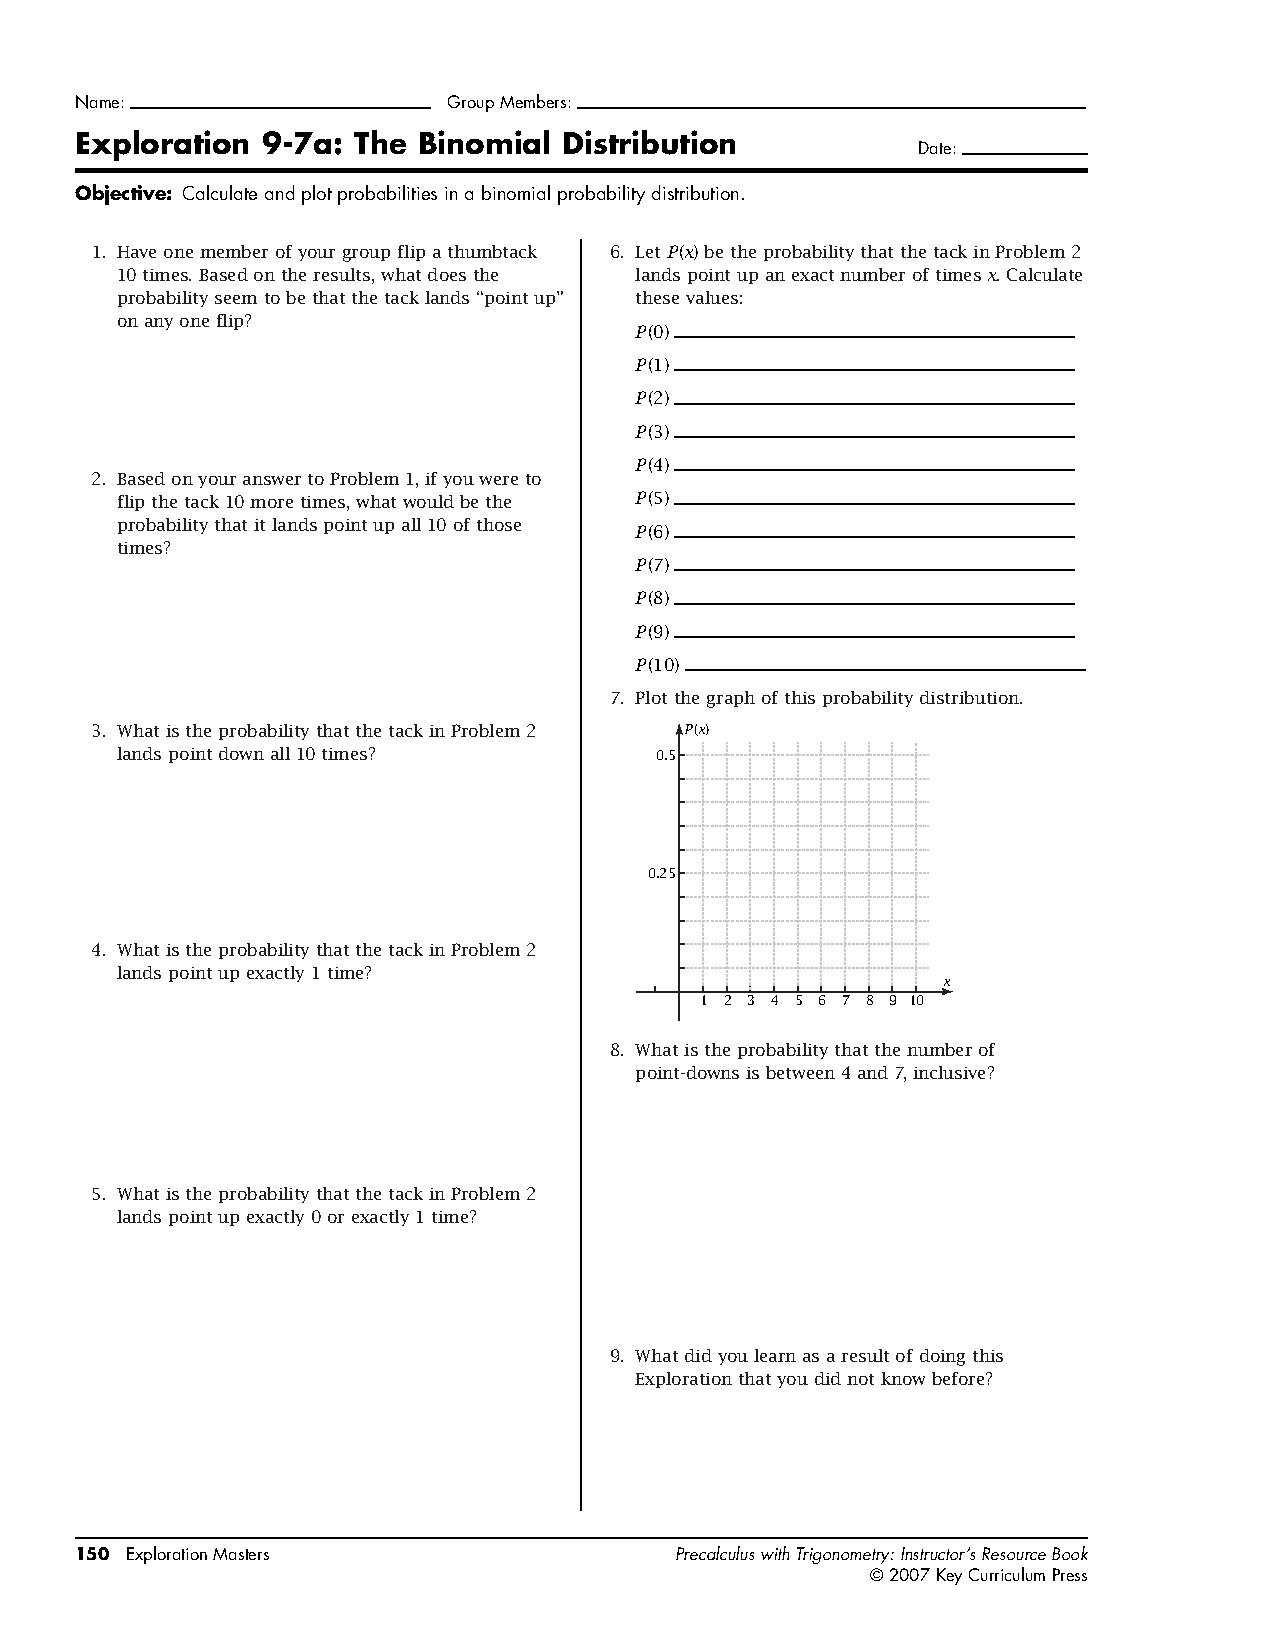
\includegraphics[width=\paperwidth]{ch14/1405p.pdf}}
\subsection{Sigma Notation}
\subsection{Binomial Probability}
\subsection{Exercises}

%									14 - 6
\newpage
\section{Review}
\subsection{Chapter Review}
\subsection{Chapter Test}

